\section{STM32 integration of eFMUs}\label{sec:STM32-integration-of-eFMUs}

The \controller{} and \plant{} eFMUs generated in Section \ref{sec:efmuGenAndSiL} still need to be system integrated on physical microcontrollers. The STM32 (STMicroelectronics\regtm{}) ecosystem has been used as the target here since it is widely-used, low-priced, and well-documented with good development and software support. Being mainly a hardware manufacturer---and as often the case in the embedded domain---STMicroelectronics' viewpoint starts from the hardware and not the model. System integration starts with the selection of one of the target microcontrollers in STM32CubeMX, where peripherals like GPIO pins, DACs, and timers are configured, with template code ultimately being generated, initializing and provisioning all configured peripherals based on the hardware abstraction layer (HAL), lower-layer (LL) drivers, and Arm\regtm{} Cortex\regtm{}-M CMSIS provided by the used STM32CubeH7 software package managed\footnote{STM32CubeMX proposes a catalog of locally installed and online available STM32CubeH7 versions suited for the target microcontroller.} in STM32CubeMX. The result of STM32CubeMX template generation is a C development project for STM32CubeIDE, whose \texttt{main()} execution routine (\texttt{int main(void)} function in \texttt{main.c}) is ready for adding the actual user-code interacting with the configured peripherals. In our case, eFMI system integration therefore means to integrate the 32-bit floating-point precision production codes of the \controller{} and \plant{} eFMUs into the \texttt{main()} execution routines of their respective template codes generated by STM32CubeMX. Note the plural; \controller{} and \plant{} have their individual STM32CubeIDE projects.

A direct STM32 system integration not using tooling like STM32CubeMX and STM32CubeIDE would be possible too, but that requires professional knowledge we consider rare in our development process, which is driven by the modeling community; it also would be a laborious task not paying off for sporadic use-cases.

\subsection{Board configuration with STM32CubeMX}\label{sec:STM32CubeMX}

\paragraph{Hardware configuration:} Two STM32 Nucleo-64/144 boards were chosen for deploying the eFMU production codes developed in Section \ref{sec:efmuGenAndSiL}. A NUCLEO-L476RG was used to deploy the \controller{}, where the system clock of 80 MHz was sufficient to support real-time evaluation of the model. A NUCLEO-H723ZG was selected to run the \plant{}. The much higher 550 MHz system clock is preferable for performing the fast matrix algebra required by the corresponding production code. Both the NUCLEO-L476RG and the NUCLEO-H723ZG have (at least) one analog input (ADC) and one analog output (DAC) for mapping the input and output signals.

\paragraph{Pin configurations:} The analog and digital I/O must be mapped to prevent peripheral collisions and minimize latency during the 5 kHz execution loop (i.e., 0.2 ms sampling period). Digital LEDs are employed to signal real-time violation and production code errors, whereas digital output pins are enabled to examine execution times through an oscilloscope by means of low/high voltage toggling at each sampling point and a separate high-voltage signal whenever eFMU production code is in execution. Digital inputs, such as the onboard push-button for the manually controlled \plant{} fault condition trigger, were also mapped in the STM32CubeMX configuration. For example, for the NUCLEO-H723ZG used for the \plant{}, the primary analog input (the voltage output of the PSS \controller{} board) was assigned to GPIO pin \texttt{PA3}, corresponding to ADC1 channel 15; and the calculated speed output ($\omega$) was assigned to GPIO pin \texttt{PA5}, which connects directly to the DAC1 output channel. A similar approach was taken for the \controller{} I/O configuration, whose NUCLEO-L476RG pin configuration is shown in Figure \ref{fig:cubemx-pin-config}.

\begin{figure}[t!]
    \vspace{-4ex}
    \centerline{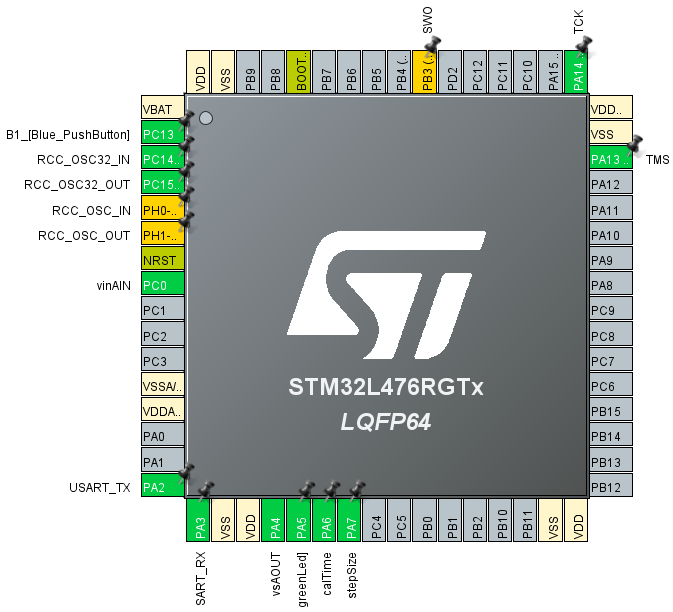
\includegraphics[width=0.9\columnwidth]{./figures/CubeMX_Pins.png}}
    \vspace{-2ex}
    \caption{STM32CubeMX pin configuration for the NUCLEO-L476RG used as the \controller{}.}
    \label{fig:cubemx-pin-config}
    \vspace{-2ex}
\end{figure}

We also prototyped more advanced plant models supporting variable loads via an additional input that can be interactively changed with a potentiometer\footnote{Although not further discussed for space considerations, the variable-load variant has been successfully deployed and tested.}. In that case, the additional analog input has been deliberately mapped to GPIO pin \texttt{PC0} because it can physically route to an entirely independent analog-to-digital converter, ADC2 (specifically \texttt{ADC123\_INP10}). Distributing the analog input signals across separate, dedicated ADCs avoids the need for complex ``Scan Mode'' channel switching or Direct Memory Access (DMA) pipelines. This hardware-level isolation ensures deterministic, low-latency sampling within the tight 0.2 ms timer interrupt.

\paragraph{Clock configurations:} In Dymola, the sampling period of eFMU configurations is explicitly set (see Section \ref{sec:eFMU-configurations}). For the STM32CubeMX configurations, the clock dividers and pre-dividers must be calculated to match the exact sampling period set in the eFMU. The timer's clock rate (its frequency) is determined by the following equation:

\begin{equation*}
    \text{frequency} = \frac{\text{APB Clock}}{(\text{ARR}+1)(\text{PSC}+1)}
\end{equation*}

\noindent{}where ARR stands for Auto-Reload Register and PSC stands for the timer's prescaler. The APB Clock is the system clock that has been pre-divided for the peripherals (such as timers). The limitations of the ARR and prescaler will be displayed in the STM32CubeMX GUI. 

For example, the embedded board that is used as the \plant{} is required to sample every 0.2 ms (i.e., at 5 kHz frequency). To this end, the NUCLEO-H723ZG, which has a 550 MHz system clock, is configured to have an APB pre-divider of 2, an ARR of 199, and a PSC of 274. That results in the desired frequency:

\begin{equation*}
    \text{frequency} = \frac{550/2 \text{ MHz}}{(199+1)(274+1)} = 5 \text{ kHz}
\end{equation*}

\noindent{}These clock configuration parameters are set in the timer peripheral menu of STM32CubeMX. For the \plant{} board, TIM2 was used with the parameters found above, as shown in Figure \ref{fig:cubemx-timer-config}.

The timer configuration for the \controller{} is likewise, except that TIM1 is used instead of TIM2 and that its APB Clock, ARR, and PSC values are different to achieve a 0.2 ms sampling period because the NUCLEO-L476RG has a 80 instead of a 550 MHz Arm Cortex-M processor.

\begin{figure}[t!]
    \centerline{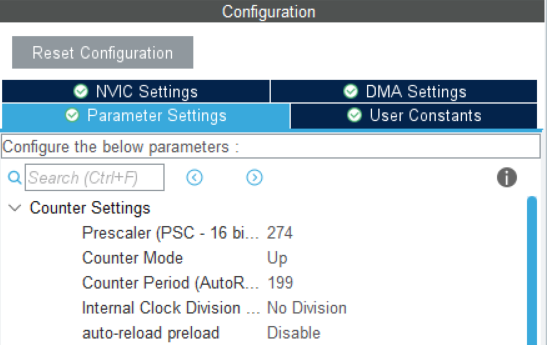
\includegraphics[width=0.9\columnwidth]{./figures/CubeMX_TIM2Config_H723.png}}
    \caption{SMT32CubeMX timer configuration for the NUCLEO-H723ZG used as the \plant{}.}
    \label{fig:cubemx-timer-config}
    \vspace{-2ex}
\end{figure}

\paragraph{Code generation configurations:} To maintain a clean file structure---in particular for the generated \texttt{main()} execution routine in \texttt{main.c}---the code generator of STM32CubeMX was set to generate peripheral initialization as a pair of \texttt{.c/.h} files per peripheral. The respective setting is in Project Manager $\rightarrow$ Code Generator $\rightarrow$ ``Generate peripheral initialization as a pair of \texttt{.c/.h} files per peripheral''. Additionally, the target IDE was set to STM32CubeIDE under Project Manager $\rightarrow$ Project $\rightarrow$ Toolchain/IDE.

\paragraph{Generated template code overview:} The template code generated by STM32CubeMX serves as the foundational bare-metal layer for the microcontrollers. Upon boot, the code initializes the ARM Cortex-M processor and configures the system clock tree to drive the NUCLEO-H723ZG at 550 MHz and the NUCLEO-L476RG at 80 MHz. The GUI shows which specific GPIO pins can be mapped to ADC and DAC channels, and initializes the hardware timers using the ARR and PSC values calculated to ensure that the timer interrupts fire at the exact 5 kHz rate required by each of the sampling periods configured in Section \ref{sec:eFMU-configurations}. In addition, initialization code for the HAL is generated. Because the eFMU's production code is system integrated into the generated template code, it is critical that all custom logic, like eFMU function calls, is placed strictly within the designated \texttt{/* USER CODE BEGIN /} and \texttt{/ USER CODE END */} tags; otherwise, code regeneration during subsequent hardware reconfigurations would overwrite the manually added production code integration.

\subsection{Programming, compilation, and deployment with STM32CubeIDE}\label{sec:STM32CubeIDE}

\paragraph{eFMU production code inclusion:} Rather than manually copying the production codes generated for the \controller{} and \plant{} into their respective STM32CubeIDE projects, the Production Code containers of the respective eFMUs were symbolically linked using relative paths based on project environment variables provided by STM32CubeIDE (e.g., \texttt{PARENT-3-PROJECT\_LOC} for the level-3 parent directory of the project root directory). This allows the \controller{} and \plant{} Modelica source models to be iteratively tweaked and re-exported from Dymola as eFMUs without requiring manual production code re-import in their respective STM32CubeIDE projects (just refreshing the projects is sufficient)---an important feature for iterative, rapid prototyping cycles from a Modelica model to deployable embedded code. Besides symbolic linking, the eFMU production codes also have to be added to the list of include and source file directories such that STM32CubeIDE takes care of their compilation and binary code generation.

\paragraph{Manual system integration in \texttt{main.c}:}\label{sec:stm32-system-integration-main-loop}

Manual coding to system integrate the eFMU production codes is only required in the \texttt{main.c} files generated by STM32CubeMX. The required steps are very similar for the \controller{} and \plant{} and are explained in the following by the example of the \controller{}.

First, the eFMU production code must be included via \texttt{\#include "block.h"} to enable \controller{} initialization, recalibration, and sampling via the eFMI GALEC block-interface routines \texttt{Startup()}, \texttt{Recalibrate()}, and \texttt{DoStep()}. Note that the implementation generated by Dymola uses hashed names, such that name clashes when several eFMUs are compiled and linked together are avoided. This is not required in our example---after all \controller{} and \plant{} are individual STM32CubeIDE projects deployed on individual boards---for which reason we can introduce simplified names via \texttt{\#define} preprocessor macros that ease the readability of subsequent system integration code:

\begin{lstlisting}[
    language = c,
    caption={},
    label={lst:main-1}]
/* USER CODE BEGIN Includes */
#include "block.h"
/* USER CODE END Includes */

/* USER CODE BEGIN PTD */
#define CONCAT_INNER(a, b) a##b
#define CONCAT(a, b) CONCAT_INNER(a, b)

/* Shortcut names for hash-based eFMU API: */
#define MODEL_HASH \
  H225c1baf6cf5a31bc9b0c38998c...

typedef CONCAT(BlockState_, MODEL_HASH) \
  ModelPSS;
typedef CONCAT(SPE_Real_, MODEL_HASH) \
  PSS_Real;
typedef CONCAT(SPE_ErrorSignal_, MODEL_HASH) \
  PSS_ErrorSignal;

#define PSS_NONE_ERRORSIGNAL \
  CONCAT(SPE_ERRORSIGNAL_NONE_, MODEL_HASH)
#define PSS_UNSPECIFIED_ERRORSIGNAL \
  CONCAT(SPE_ERRORSIGNAL_UNSPECIFIED_ERROR_, MODEL_HASH)

#define PSS_Startup \
  CONCAT(Startup_, MODEL_HASH)
#define PSS_DoStep \
  CONCAT(DoStep_, MODEL_HASH)
#define PSS_Recalibrate \
  CONCAT(Recalibrate_, MODEL_HASH)
#define PSS_Reinitialize \
  CONCAT(Reinitialize_, MODEL_HASH)
/* USER CODE END PTD */
\end{lstlisting}

\noindent{}Next, two global variables are introduced to capture sampling requests of the timer interrupt (\texttt{pending\_samplings}) and to engage or disengage the \controller{} interactively (\texttt{use\_pss}); the latter will be used in Section \ref{sec:results-and-analyses} to validate the stabilizing effects of the \controller{}:

\begin{lstlisting}[
    language = c,
    caption={},
    label={lst:main-2}]
/* USER CODE BEGIN PV */
/* Sampling request counter & PSS on/off button: */
static volatile uint8_t pending_samplings;
static volatile bool use_pss;
/* USER CODE END PV */
\end{lstlisting}

\noindent{}Note that both variables are \texttt{volatile} since they shall be changed by interrupt routines\footnote{There is no need for semaphores because the single core ARM Cortex-M processor guarantees atomic access for \texttt{uint8\_t} and \texttt{bool}.}; the \texttt{pending\_samplings} variable is changed whenever the timer interrupt triggers and \texttt{use\_pss} whenever the \texttt{B1} onboard button shown in Figure \ref{fig:wiring-diagram} is pressed. The interrupt routines we need to adapt are predefined by the STM32 HAL; \texttt{HAL\_TIM\_PeriodElapsedCallback} for the timer and \texttt{HAL\_GPIO\_EXTI\_Callback} for the onboard button:

\begin{lstlisting}[
    language = c,
    caption={},
    label={lst:main-3}]
/* USER CODE BEGIN 4 */
void HAL_TIM_PeriodElapsedCallback(
  TIM_HandleTypeDef *htim)
{
  /* Check for sampling timer interrupt: */
  if (TIM1 == htim->Instance)
  {
    if (((uint8_t) 255) > pending_samplings)
    {
      ++pending_samplings;
    }
    HAL_GPIO_TogglePin(
      stepSize_GPIO_Port,
      stepSize_Pin);
  }
}

void HAL_GPIO_EXTI_Callback(uint16_t GPIO_Pin)
{
  static uint32_t last_override = ((uint32_t) 0);

  /* Check for blue button (PC13) interrupt: */
  if (B1__Pin == GPIO_Pin)
  {
    const uint32_t current_time = HAL_GetTick();
    /*
      Debounce; only accept press if 250 ms
      passed since last:
    */
    if (((uint32_t) 250)
      < (current_time - last_override))
    {
      use_pss = !use_pss;
      last_override = current_time;
    }
  }
}
/* USER CODE END 4 */
\end{lstlisting}

\noindent{}The checks on Lines~6 and 23 are based on our STM32CubeMX \controller{} configuration for the timer (\texttt{TIM1}) and onboard button (\texttt{B1\_\_Pin}) peripherals, and ensure the action is only taken if the respective peripheral caused the interrupt. In case of the timer, we simply increase the \texttt{pending\_samplings} on Line~10 (ensuring it saturates instead of overflowing); in case of interactive \controller{} toggling we just invert \texttt{use\_pss} on Line~33 (incorporating a debounce time to avoid toggle-cascading).

We also flip a digital output on Lines~12-14 whenever the timer ticks. The resulting \texttt{stepSize} pulse signal---whose fixed-length is the sampling period---is useful for the computation time analyses of Section \ref{sec:results-and-analyses} since it provides a reference-grid for oscilloscope-based plots of the time required by the eFMU production code for computing individual samplings (cf. \texttt{calTime} of the control-loop listing below).

ARM Cortex-M interrupt routines have defined priority levels. Only routines of higher priority can interrupt others; pending interrupts of lower or equal priority are delayed until higher priority interrupts are complete. The logic of interrupt routines therefore should be concise to avoid interrupt overruns. For that reason, our timer interrupt only registers another sampling request in \texttt{HAL\_TIM\_PeriodElapsedCallback} instead of conducting the actual sampling (which would, in case of an overrun, silently block a following timer tick). The sampling code itself is within the control-loop of the interruptible \texttt{main()} execution routine:

\begin{lstlisting}[
    language = c,
    caption={},
    label={lst:main-4}]
/* USER CODE BEGIN WHILE */
while (true)
{
  /* USER CODE END WHILE */

  /* USER CODE BEGIN 3 */
  /* Conduct sampling if sampling timer ticked: */
  if (((uint8_t) 0) < pending_samplings)
  {
    /* Always reset the error signals: */
    error_signals = PSS_NONE_ERRORSIGNAL;

    /* Computation time for external profiling: */
    HAL_GPIO_WritePin(
      calTime_GPIO_Port,
      calTime_Pin,
      GPIO_PIN_SET);

    /* Input processing (convert AC to volt): */
    HAL_ADC_Start(&hadc1);
    if (HAL_OK == HAL_ADC_PollForConversion(
      &hadc1,
      POLL_TIMEOUT))
    {
      const uint32_t adc_raw =
        HAL_ADC_GetValue(&hadc1);
      pss.vSI =
        ((PSS_Real) adc_raw) * ADC_TO_VOLTS;
    }
    else
    {
      error_signals |= PSS_UNSPECIFIED_ERRORSIGNAL;
    }
    HAL_ADC_Stop(&hadc1);

    /* Compute sampling step: */
    PSS_DoStep(&pss);
    error_signals |= pss.ErrorSignals;

    /* Check if switch is pulling to GND: */
    const PSS_Real target_pu = use_pss
      ? pss.vs
      : CONSTANT_PU;

    /*
      Output processing (scaling, clamping,
      converting volt to AC):
    */
    PSS_Real dac_val =
      (target_pu + OFFSET) * VOLTS_TO_DAC;
    if (DAC_MIN > dac_val)
    {
      dac_val = DAC_MIN;
    }
    else if (DAC_MAX < dac_val)
    {
      dac_val = DAC_MAX;
    }
    HAL_DAC_SetValue(
      &hdac1,
      DAC_CHANNEL_1,
      DAC_ALIGN_12B_R,
      ((uint32_t) dac_val));

    /* Computation time for external profiling: */
    HAL_GPIO_WritePin(
      calTime_GPIO_Port,
      calTime_Pin,
      GPIO_PIN_RESET);

    --pending_samplings;
  }

  /* Set LED 2 for sampling errors or overruns: */
  if ((PSS_NONE_ERRORSIGNAL != error_signals)
    || (((uint8_t) 1) < pending_samplings))
  {
    error_timestamp = HAL_GetTick();
    HAL_GPIO_WritePin(
      LD2__GPIO_Port,
      LD2__Pin,
      GPIO_PIN_SET);
  }

  /*
    Unset LED 2 if on due to past errors
    (but always hold for at least 30000 ms):
  */
  if ((((uint32_t) 0) != error_timestamp)
    && (((uint32_t) 30000)
      < (HAL_GetTick() - error_timestamp)))
  {
    HAL_GPIO_WritePin(
      LD2__GPIO_Port,
      LD2__Pin,
      GPIO_PIN_RESET);
    error_timestamp = ((uint32_t) 0);
  }
}
/* USER CODE END 3 */
\end{lstlisting}

\noindent{}Note that the control-loop is greedy (\texttt{while (true)} on Line~2) instead of going to sleep until events happen; such ``busy waiting'' is typical for hard real-time code. It consists of three main parts: (1) On Lines~8-72, actual sampling---i.e., the use of eFMU production code to compute new outputs and internal control states for the given inputs and parameters---is conducted whenever the timer interrupt indicated a sampling point (\texttt{pending\_samplings} $\geq$ 1). (2) On Lines~75-83 errors---either (a) signaled by the block-interface functions of the eFMU production code (\texttt{error\_signals} variable set on Lines~37-38) or due to real-time violations, because of (b) non-timely input provision (timeout of \texttt{HAL\_ADC\_PollForConversion} on Lines~21-23) or (c) sampling computation overruns when the timer ticks again while a previous sampling still is processed (\texttt{pending\_samplings} $>$ 1 check on Line~76)---are detected and indicated by the onboard LED 2. (3) On Lines~89-98, LED 2 is reset if there have been no errors within the last 30 s.

Note that sampling on Lines~8-72 is mostly about input and output provisioning with respective timeout detection and AC/voltage conversions with scaling and clamping according to voltage ranges. The actual sampling logic is completely encapsulated in the eFMI \texttt{DoStep()} implementation of the eFMU production code (called on Line~37), which takes as argument a struct holding the current \controller{} state (\texttt{pss} holding the values of tunable and dependent parameters, in- and outputs, and states). The struct type is provided by the eFMU production code as is a respective eFMI \texttt{Startup()} implementation for its initialization. The only other noteworthy sampling actions are (1) to indicate the actual computation time with the \texttt{calTime} pulse signal (set to high-voltage when sampling starts on Lines~14-17 and reset on Lines~66-69 when it ends), (2) engage or disengage---not disable; just whether its output shall be used---the \controller{} on user request on Lines~41-43, and, of course, (3) reduce the sampling request counter on Line~71 when finished.

\paragraph{Compiler and linker settings:}

STM32CubeIDE provides various options for compilation and binary code generation. Our \controller{} and \plant{} projects each provide two predefined build configurations: A \textit{Debug} and a \textit{Release} build. Both share the following common settings (unmentioned options are left default):

\squishlist
    \item \textbf{MCU/MPU Toolchain:} The GNU Tools for STM32 (14.3.rel1) are used for compilation and binary code generation.
    \item \textbf{MCU/MPU Settings:} Use of the reduced C runtime library (\texttt{--specs=nano.specs}) and hardware-implemented floating-point ABI (\texttt{-mfloat-abi=hard}). For the NUCLEO-L476RG, where the \controller{} is deployed, its FPv4-SP-D16 floating-point unit is used; for the NUCLEO-H723ZG, its FPv5-D16 floating-point unit is used.
    \item \textbf{MCU/MPU GCC Assembler:} The preprocessor does not search system directories (\texttt{-nostdinc}) to avoid inclusion or configuration by external---third party set---macros.
    \item \textbf{MCU/MPU GCC Compiler:} Reports are verbose (\texttt{-v}). ISO C18 (\texttt{-std=c18}) is used as language standard to verify portability and compliance of the eFMU production code generated by Dymola. All warnings are enabled (\texttt{-Wall}, \texttt{-Wextra}, \texttt{-pedantic}, \texttt{-Wmissing-include-dirs}, \texttt{-Wswitch-default}, \texttt{-Wswitch-enum}, and \texttt{-Wconversion}). As expected from the production code analyses of Section \ref{sec:production-code-quality-analyses}, the eFMU production codes are free of any warnings except the 32-bit floating-point narrowing conversions already explained; interestingly, the driver/standard library implementation of STM32 has many warnings.
    \item \textbf{MCU/MPU GCC Linker:} Reports are verbose (\texttt{-v}). Standard libraries are not default included (\texttt{-nodefaultlibs}) and a minimal implementation for system calls is used (\texttt{--specs=nosys.specs}) to verify that the eFMI production code generated by Dymola is self-contained and without external library dependencies besides basic C Standard Library dependencies.
\squishend

\noindent{}The \textit{Debug} and \textit{Release} builds only differ in applied optimizations and available debug support:

\squishlist
    \item \textbf{MCU/MPU GCC Assembler:} The debug level is maximum (\texttt{-g3}) for the \textit{Debug} build and none for the \textit{Release} build; likewise for the MCU/MPU GCC Compiler settings, where additionally the \texttt{-DDEBUG} preprocessor directive is defined for the \textit{Debug} build but not for the \textit{Release} build.
    \item \textbf{MCU/MPU GCC Compiler:} The optimizations are none (\texttt{-O0}) for the \textit{Debug} build and most (\texttt{-O3}) for the \textit{Release} build. Stack usage analysis (\texttt{-fstack-usage}) and cyclomatic complexity (\texttt{-fcyclomatic-complexity}) are enabled for the \textit{Debug} build but not for the \textit{Release} build.
\squishend
